\chapter{Work Plan}
\label{chap:workplan}
In order to accomplish the goals described in \autoref{sec:goals} several work needs to be done.
This chapter presents the several task under which the work has been split into.
Those cover the basic literature review and study, developing, testing, evaluation and writing the final report and presentation of this thesis.

\section{Tasks Description}
\subsection{Literature Review}
Although during the preparation of this report several concepts and theories were already studied, during the thesis they will need to be deeper analysed and studied.
This task is expected to be spread out during the whole thesis preparation though with a bigger impact in the beginning.

\subsection{Study Property-base semantic mapping system}
Adding to the base literature review, the novel proposed system \cite{pronobis2011exploiting} requires additional study and understanding as one of the focus of this thesis is the evaluation of that system. This will be one of the first tasks to be completed.

\subsection{Implement novelty detection algorithms}
As described in \autoref{sec:approach-novelty} novelty detection can be seen as two separate methods.
Those two methods will be implemented, starting with the identification of novel room types directly on the \emph{graphical model}.
Later the graphical model will be expanded to be able to handle novelty signals from the classifiers used to extract sensed properties.

\subsection{Testing and Evaluation of developed methods}
A step of this thesis is an evaluation of the used approach and determination of its efficiency.
The developed methods will be run through the databases described in \autoref{sec:databases}.

The results will be compared and used for tunning parameters and redirect research efforts.
For final evaluation and comparison the developed method will be submitted to robot task of \gls{ImageCLEF}.

\subsection{Thesis Writing}
As final stage all the study and results will be written in the Master thesis and its presentation will be prepared.

\section{Tasks Schedule}
Due to the nature of the tasks at hand its impossible to predict exact dates or give precise and detailed description on each of them.

We point to the fact that novelty research on itself is not an easy topic as it requires specific knowledge to each case. And also the approaches detailed here are novel on itself and its impossible to predict the problems that may appear as we move forward on the research.

Its however possible to give an high-level level overview of the tasks and their order of execution.
As presented on the graph below:
\begin{figure}[!h]
\center
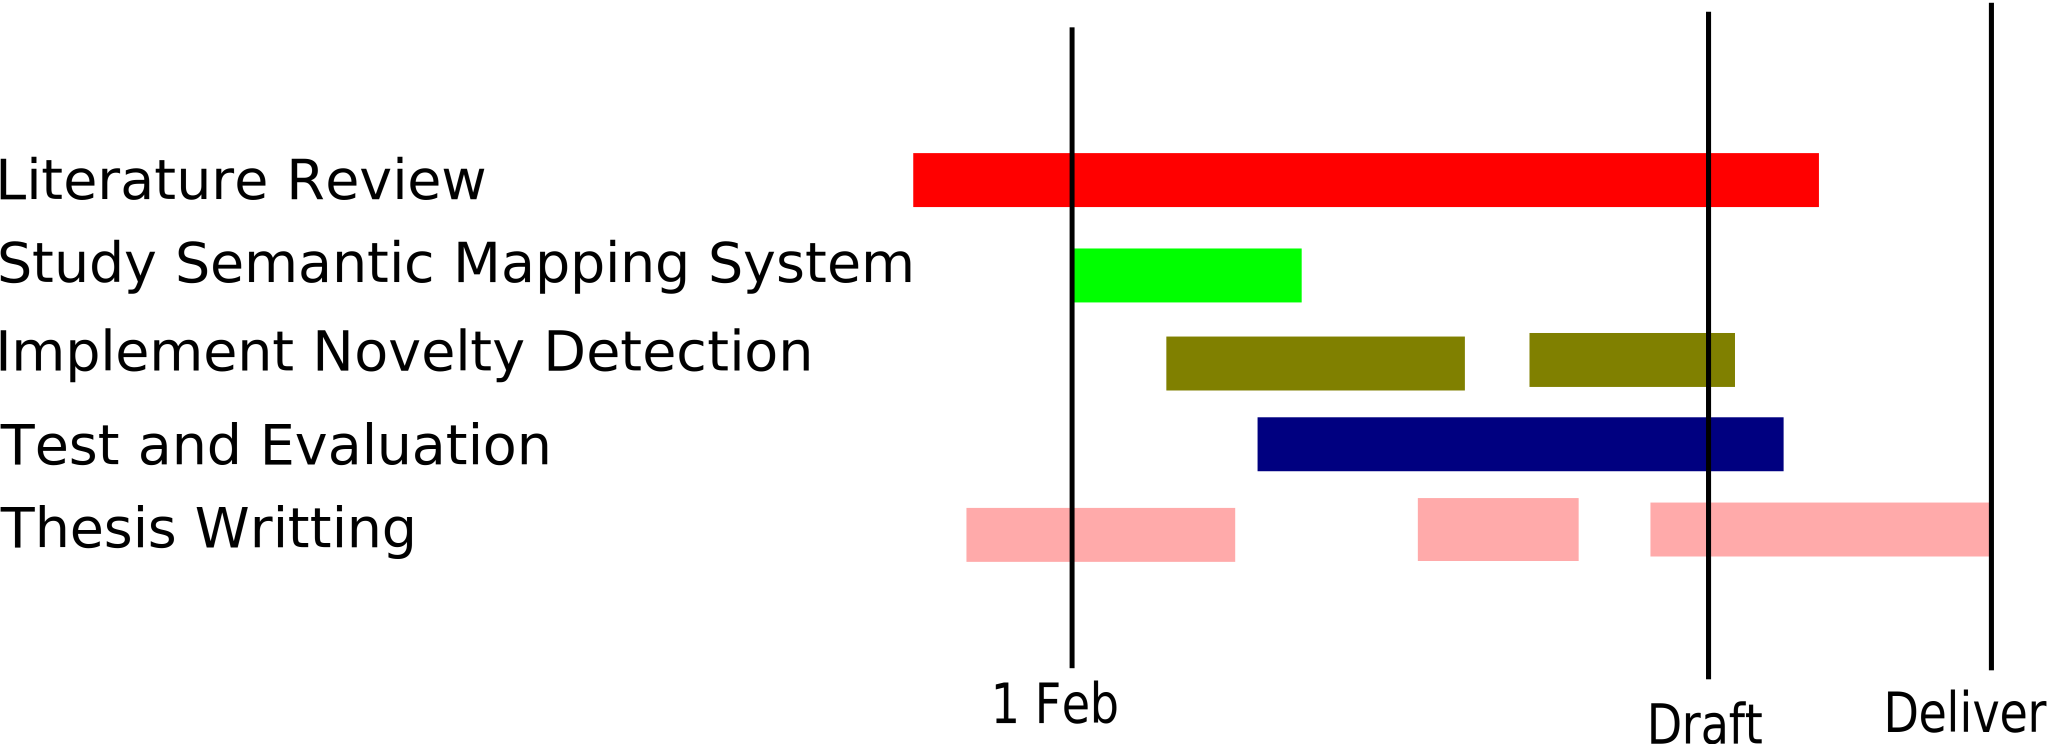
\includegraphics[width=\linewidth]{gantt.pdf}
\caption{Scheme of tasks to be completed over time.}
\end{figure}

As shown the literature review, thesis writing and a small part of the system study were the main focus until the moment. Since that was required knowledge to the writing this report.

Next focus will be on implementation of novelty detection on top off the graphical-model. Test and evaluation also start earlier as scripts and performance measures need to be established in order to correctly implement the developed methods. Some writing will be involved after that in order to report results on the developed method.

After that focus will be on integration of novelty detection at the level of properties classifiers. And respective changes on the graphical-model to handle that additional information provided by the classifiers.

At last efforts will be redirected to the conclusion of the thesis writing and preparation of its presentation.

